\cleardoublepage

\chapter{Study 3. DRF, cognitive abilities, and default mode network}
\label{res:dmn-crea}

\cleardoublepage

\textbf{{\large High dream recall frequency is associated with increased creativity and functional connectivity in the default mode network}}

\hfill \emph{In preparation}

\bigskip

Raphael Vallat\textsuperscript{1} (PhD candidate), Alain Nicolas\textsuperscript{1,2} (M.D, PhD), Perrine Ruby\textsuperscript{1} (PhD)

\textsuperscript{1} Lyon Neuroscience Research Center, Brain Dynamics and Cognition team, INSERM UMRS 1028, CNRS UMR 5292, Université Claude Bernard Lyon 1, Université de Lyon, Lyon, France

\textsuperscript{2} Unité Michel Jouvet, Centre Hospitalier Le Vinatier, 95 boulevard Pinel, Lyon, France

\subsection*{Summary}
\label{res:dmn-crea:summary}
Several results suggest that the frequency of dream recall is positively correlated with personality traits such as creativity and openness to experience. These findings are coherent with neuroimaging result showing different neurophysiological profiles in high dream recallers (HR) and low dream recallers (LR).  As compared to LR, a higher regional cerebral blood flow within core regions of the default mode network has been observed in HR during sleep and wakefulness. These observations are consistent with the emerging view that dreaming and mind wandering pertain to the same family of spontaneous mental processes, subserved by the default mode network. To further test this hypothesis, we assessed in HR (n=28) and LR (n=27) the (1) functional connectivity in the default mode network during resting wakefulness using fMRI as well as (2) creative-thinking, personality traits and cognitive abilities. As expected, HR demonstrated a greater DMN connectivity than LR, higher scores of creativity, and no significant difference in cognitive or memory abilities. These results support the forebrain and the DMN hypotheses of dreaming and suggest that increased activity in the DMN promote creative-thinking during both wakefulness and sleep.

\paragraph{Keywords}
Dream recall, creativity, resting state, functional connectivity, default mode network

\subsection*{Introduction}
\label{res:dmn-crea:intro}
Despite recent advances, the cerebral mechanisms favoring the production or memory of dreams are still poorly understood (see \citealp{ruby_experimental_2011}). While dreaming has long been equated with rapid eye movement (REM), it is now well established that dreaming can also occur in any sleep stages and is therefore not exclusive to a specific functional brain state. Since it is impossible to know for sure when one is actually dreaming while asleep, most empirical investigation of dreaming are therefore based on the study of dream report after awakening the dreamer \citep{schwartz_dreaming:_2005}.

As a consequence, neurophysiological studies on dreaming have either focused on comparing the brain activity in the minutes preceding an awakening associated with the presence or absence of dream recall \citep{esposito_reduced_2004, wittmann_nrem_2004, chellappa_cortical_2011, marzano_recalling_2011, scarpelli_state-_2015, siclari_neural_2017}, or on investigating the cognitive and brain functioning associated with high or low dream recall frequency (DRF; \citealp{eichenlaub_brain_2014, eichenlaub_resting_2014}).

With respect to the second line of research, recent works from our team highlighted several neurophysiological differences between high dream recallers (HR) and low dream recallers (LR), not only during sleep but also during wakefulness \citealp{eichenlaub_brain_2014, eichenlaub_resting_2014, vallat_increased_2017}. For instance, we compared using PET the spontaneous regional cerebral blood flow (rCBF) of HR and LR during sleep and wakefulness, and showed that HR have a higher spontaneous rCBF than LR in the temporo-parietal junction (TPJ) and in the medial prefrontal cortex (MPFC) during REM sleep, N3 sleep and wakefulness \citep{eichenlaub_resting_2014}. We argued that these two regions must play a key role in dream production or recall since lesions of these same areas have been found to be consistently correlated with global or partial cessation of dream reporting (without any concurrent sleep disturbance; see \citealp{solms_neuropsychology_1997}). It is noteworthy that the MPFC and TPJ are part of the default mode network (DMN), a set of functionally-coupled brain regions which are highly activated during internally oriented mental processes and memory retrieval \citep{gusnard_searching_2001, raichle_default_2001}. This network is centered on the MPFC, the posterior cingulate cortex (PCC) and the lateral parietal (LP) areas around the TPJ area.

The finding of a higher spontaneous rCBF within core regions of the DMN in HR compared to LR provides strong evidence supporting the hypothesis of a differential cognitive and brain functioning between high and low frequency dream recallers. This idea was first put forward by \citet{schonbar_differential_1965} who postulated that high dream recall is part of a general life style characterized, inter alia, by creativity, divergent thinking and introspection. Several subsequent works confirmed this hypothesis by showing a substantial correlation between DRF and creativity \citep{fitch_variations_1989, schredl_creativity_1995, schredl_factors_2003}, and DRF and personality traits such as openness to experience \citep{hartmann_boundaries_1989, schredl_dreaming_1996, schredl_dream_2003}. These observations fit remarkably well within the emerging view that dreaming and creative-thinking are both members of a broad family of spontaneous-thought phenomena, which also includes mind-wandering and daydreaming \citep{christoff_mind-wandering_2016}. Several works indicate that dreaming and creativity could be both underpinned by a strong recruitment of the DMN, and especially the prefrontal areas \citep{domhoff_neural_2011, ellamil_evaluative_2012, jung_structure_2013, beaty_creativity_2014, mok_interplay_2014, beaty_default_2015, christoff_mind-wandering_2016}.

The main conclusion to be drawn from these studies is that high dream recall seems to be on one hand related to the spontaneous activity of the DMN, and the other hand related to a general life style involving at least higher creativity. The purpose of the present study is to go a step further by characterizing the intrinsic DMN functional connectivity of HR and LR during resting-state wakefulness, as well as measures of personality, cognitive abilities and creativity. The results highlight a greater DMN connectivity in HR which was concomitant with higher scores of creativity. These results were not associated with further group differences in cognitive or memory abilities.

\subsection*{Methods}
\label{res:dmn-crea:methods}

\subsubsection*{Participants}
Behavioral and neurophysiological data were acquired from 55 healthy subjects (28 males, mean age = 22.55, standard deviation = 2.41, range = 19–29). The subjects were informed of the study through an announcement sent to the mailing list of Lyon University, which briefly described the study and included a link to a questionnaire concerning sleep and dream habits. Subjects were selected if they reported and subsequently confirmed during a phone interview: (1) having a high or low DRF (DRF superior to 5 dream recall per week and inferior to 2 dream recall per month respectively) (2) having a regular sleep-wake schedule, no difficulty to fall asleep, being occasional or frequent nappers and having preferentially already done an MRI brain scan in the past few years. Importantly, the subjects were unaware that DRF was the main criterion for inclusion in the study.

Among the 55 participants, 28 of them were high dream recallers (HR; mean DRF = 6.6 ± 0.6 dream reports per week) and 27 were low dream recallers (LR; mean DRF = 0.2 ± 0.1 dream report per week). Apart from the DRF (p<.0001), the two groups did not differ in age, habitual sleep duration or education level (Table 1). They had no history of neurological and psychiatric disorders, and had no sleep disturbances. The local ethics committee (Centre Leon Bérard, Lyon) approved this study, and subjects provided written, informed consent in conformity with the Declaration of Helsinki. The subjects were paid for their participation.

\subsubsection*{Procedure}
This study is related to a larger combined EEG-fMRI study investigating the differences between high and low dream recallers during the minutes following awakening from a short daytime nap. On this occasion, we acquired three six minutes resting-state scans, located before, 5 min after awakening and 25 min after awakening, respectively. The procedure is detailed as follows. After lunch at 11.30 am, participants were conducted to the neuroimaging center (CERMEP). During the first half hour, experimenters installed on the participant’s head a MRI compatible EEG cap (EASYCAP®). Participants were then installed in the MRI scanner at about 1.20 pm (1.17 pm ± 13 min). The first resting-state scan was then acquired, with the instructions to remain awake and look at a central fixation cross on the screen. At the end of the scan, participants were informed that they could sleep during the next 45 min. At the end of the nap slot, participants were awakened, if they were sleeping, by calling their first name and the 2nd resting state scan was acquired. During the following 10 minutes, subjects were asked about their dream(s) and sleep in the scanner. Then the 3rd resting state scan was performed about 25 min after awakening. Finally, an 8-min T1 anatomical scan was acquired. To facilitate sleep in the MRI environment, participants were allowed to sleep between 5 am and 8 am the night before the experiment. The partial sleep deprivation took place under the constant supervision of nurses in the sleep unit of Le Vinatier Hospital.

\subsubsection*{Data collection and analysis}
\paragraph{MRI acquisition}
MRI scans were obtained from a MAGNETOM Prisma 3.0 T scanner (Siemens Healthcare, Erlangen, Germany) at the Primage neuroimaging platform (CERMEP). Structural MRI were acquired with a T1-weighted (0.9-mm isotropic resolution) MPRAGE sequence and functional MRI data with a T2*-weighted 2D gradient echo planar imaging sequence (EPI) with 180 volumes (TR/TE: 2000/ 25 ms; flip angle: 80°; voxel size: 2.68 × 2.68 × 3 mm; slices: 40, duration: 6 minutes). Functional and anatomical scans were performed using a 20-channel head coil. The coil was foam-padded to improve subject comfort and restrict head motion.

\paragraph{Behavioral tests}
In addition with neurophysiological measures, participants were presented with various tests to assess the potential between group differences at the cognitive and personality levels. These tests were administered by author R.V during the evening prior to the partial sleep deprivation. A detail description follows.

\emph{BFI}. The Big Five Inventory (BFI) is a self-report inventory designed to measure the Big Five dimensions \citep{john_big_1999}, which have been typically labelled as O (Openness to experience), C (Conscientiousness), E (Extraversion), A (Agreeableness), N (Neuroticism). We used the validated French version (BFI-Fr; \citealp{plaisant_validation_2010}), which includes 45 items presenting a collection of statements concerning interpersonal relationships and personality. Each item is scored on a 5-point Likert-type response scale, ranging from 'strongly disagree' (1) to 'strongly agree' (5).

\emph{STAI}. The State-Trait Anxiety Inventory (STAI) is a self-report inventory consisting of 40 items pertaining to anxiety affect \citep{spielberger_manual_1970}. The STAI purports to measure one's conscious awareness at two extremes of anxiety affect, labeled state anxiety (A-state), and trait anxiety (A-trait), respectively. The A-Trait and A-State scales comprise 20 items each, scored on a 4-point Likert-type response scale. Scores range from 20 to 80, with higher scores suggesting greater levels of anxiety.

\emph{PQSI}. The Pittsburgh Sleep Quality Index (PQSI) is a self-rated questionnaire which assesses sleep quality and disturbances over a one-month time interval \citep{buysse_pittsburgh_1989}. It comprises 19 individual items concerning among others subjective sleep quality, sleep latency, sleep duration and daytime dysfunction. Higher scores at the PQSI indicate poorer sleep quality.

\emph{MEM-III}. The MEM-III is the validated French version of the Wechsler Memory Scale (WMS-third edition, WMS-III; \citealp{wechsler_mem-iii:_2001}).  We used a subtest to assess immediate and delayed memory. Participants were read the first story, after which they were instructed to say out loud everything they could remember of this story. The experimenter rated how many items (maximum 25) the participants were able to recall. Twenty five minutes later, the subjects were asked again to recall the stories (delayed memory). Importantly, the subjects were not aware that they would have to recall any of the images at any point after the test. For both immediate and delayed recall, scores were averaged over the two stories and therefore range from 0 to 50, with higher scores reflecting greater memory performances.

\emph{Digit span}. Individual memory abilities were also assessed using a digit span task, which measures the working memory’s number storage capacity. Participants were asked to repeat a heard sequence of numerical digits, the length of which increases at each trial. Digit span was assessed first forwards (maximum score 16) and then backwards (maximum score 14). The digit span index was obtained by averaging the two scores. Higher scores (maximum 30) indicate higher working memory abilities.

\emph{Guildford’s Alternative Uses Task}. The Guildford Uses Task \citep{guildford_alternate_1978} is a creativity test in which participants are asked to list as many possible uses for an everyday object. Participants were shown images of three objects (a pen, a mug, a chair) in a randomized order and subsequently asked to list, during 2 minutes, as many alternative or unusual uses for this object. The fluency index is the total number of responses averaged across the three items. Higher scores indicate higher creativity. Additionally, we computed for each subject and each item the number of rare uses (top 10\% rarest uses, i.e. uses found by 5 or less participants). The rare uses index is the total number of rare uses averaged across the three items. Higher scores indicate higher creativity.

\paragraph{fMRI analysis}
One subject (HR) was excluded from the MRI analysis because of a technical failure during MRI acquisition, leading to a total of 27 HR and 27 LR. As the failure only concerned MRI acquisition, the behavioral and cognitive measures of this participant were still included in the analysis. For the remaining subjects, preprocessing and quality check were performed using standard routine in SPM12 software (Wellcome Department of Imaging Neuroscience). Preprocessing included functional realignment, slice-time correction, coregistration to structural scan, spatial normalization and spatial smoothing using a 6 mm full-width at half-maximum isotropic Gaussian kernel filter. Individual T1 images were segmented into gray matter, white matter and cerebrospinal fluid tissue maps. Functional and structural images were then normalized to MNI152 space (Montreal Neurological Institute). Functional images underwent artifact and motion regression in the Artifact Detection Toolbox using the following criteria to define outliers: global signal intensity changes greater than 9 standard deviations and movement exceeding 2 mm. SPM motions parameters and outliers were subsequently included as covariates in connectivity analyses.

Connectivity analysis were performed on the concatenated resting-state scans (3 scans x 6 minutes = 18 minutes resting-state data) using the CONN toolbox version 17f \citep{whitfield-gabrieli_conn:_2012}. As the aim of this study was to compare the DMN connectivity during resting-state between HR and LR, we selected 4 main regions of interests (ROIs) corresponding to the core nodes of the DMN (see Fig 1A). These include the Posterior Cingulate Cortex (PCC; center of mass in MNI coordinates: 1, -61, 38), the Medial Prefrontal Cortex (MPFC; 1, 55, -3) and bilateral Lateral Parietal cortices (LP; left: -39, -77, 33, right: 47, -67, 29). These regions are implemented within the CONN Toolbox version 17f as part of a parcellation atlas of the main brain networks, obtained by applying an independent component analysis on 467 subjects from the Human Connectome Project.

The connectivity analysis included the following steps: first, we performed a denoising step including a regression of the 6 motion correction parameters and their corresponding first-order temporal derivatives, as well as a component-based strategy (aCompCor, \citealp{behzadi_component_2007}) to identify and remove physiological confounds that are unlikely to be related to neural activity. The resulting BOLD time series were band-pass filtered (0.008 – 0.09 Hz) to further reduce noise and increase sensitivity \citep{weissenbacher_correlations_2009}. Then, Pearson’s correlation coefficients were calculated for each pair-wise connection across the 4 nodes of the DMN, resulting in a single skew-symmetric connectivity matrix with 6 correlation coefficients for each subject. These values were normalized using a Fisher’s r-to-Z transformation and then compared between HR and LR (two-sided t-tests corrected for multiple comparisons using the false discovery rate (FDR, p<.05)). Finally, the mean DMN connectivity (average of all pair-wise correlations) was calculated and compared between groups.

\paragraph{Statistics}
As several studies reported a higher creativity in HR than in LR, between group comparisons of the fluency index and rare uses index were achieved using one-tailed T-test (p<.05). Similarly, as we expected HR to demonstrate a higher DMN functional connectivity than LR, between group statistical comparisons of the mean DMN functional connectivity was achieved using one-tailed T-test. All the other comparisons were achieved using two-sided T-tests.

\subsection*{Results}
\label{res:dmn-crea:results}

\clearpage

\setlength\LTleft{0pt}
\setlength\LTright{0pt}
\renewcommand{\arraystretch}{.9}
\begin{longtable}{@{\extracolsep{\fill}}lllllll@{}} % xlxllxx
    \caption*{\textbf{Table 1. Subject information.} DRF: habitual weekly dream recall frequency (the number of awakenings per week with a dream in mind). Gender: subject’s gender (F, female; M, male). Age: subject’s age (years). Sleep duration: habitual sleep duration during the week (hours). Education: number of years of education. Age, habitual sleep duration and education level were not significantly different between High-recallers and Low-recallers; however, the DRF was significantly larger in High-recallers than in Low-recallers (t-test, ***P<0.0001).} \\
    \toprule
	Group          	& N° & DRF            & Gender & Age  			& Sleep duration	& Education       \\ \midrule
	High recallers 	& 1  & 6              & M      & 19.3 			& 7             	& 0               \\
	               	& 2  & 7              & M      & 23.9 			& 8             	& 3               \\
	               	& 3  & 7              & M      & 22.6 			& 8             	& 4               \\
	               	& 4  & 7              & F      & 21.0 			& 9             	& 3               \\
	               	& 5  & 7              & F      & 24.1 			& 8.3           	& 5               \\
	               	& 6  & 7              & F      & 19.4 			& 7.5           	& 1               \\
	               	& 7  & 5              & F      & 23.7 			& 8.33          	& 4               \\
	               	& 8  & 7              & M      & 23.8 			& 8             	& 3               \\
	               	& 9  & 6              & M      & 27.2 			& 7.5           	& 8               \\
	               	& 10 & 7              & M      & 23.9 			& 8             	& 5               \\
	               	& 11 & 7              & F      & 18.9 			& 9             	& 1               \\
	               	& 12 & 7              & F      & 24.2 			& 8.5           	& 5               \\
	               	& 13 & 6              & M      & 23.0 			& 6             	& 5               \\
	               	& 14 & 6              & F      & 21.1 			& 8.5           	& 3               \\
	               	& 15 & 7              & F      & 20.6 			& 8.5           	& 3               \\
	               	& 16 & 6              & M      & 28.1 			& 7             	& 9               \\
	               	& 17 & 7              & F      & 19.6 			& 8             	& 1               \\
	               	& 18 & 7              & F      & 23.9 			& 7             	& 5               \\
	               	& 19 & 6              & M      & 22.7 			& 9             	& 4               \\
	               	& 20 & 6              & M      & 21.8 			& 9             	& 3               \\
	               	& 21 & 7              & F      & 20.8 			& 8             	& 4               \\
	               	& 22 & 7              & M      & 26.3 			& 7             	& 4               \\
	               	& 23 & 7              & F      & 19.1 			& 8             	& 1               \\
	               	& 24 & 7              & F      & 21.1 			& 7             	& 4               \\
	               	& 25 & 7              & F      & 22.7 			& 6             	& 4               \\
	               	& 26 & 7              & F      & 23.2 			& 9             	& 5               \\
	               	& 27 & 6              & M      & 22.3 			& 8             	& 10              \\
	               	& 28 & 6              & M      & 21.0 			& 7             	& 3               \\
	Low recallers  	& 1  & 0.5            & F      & 25.3 			& 8             	& 4               \\
	               	& 2  & 0.5            & M      & 23.3 			& 8             	& 4               \\
	               	& 3  & 0              & M      & 21.0 			& 6             	& 2               \\
	               	& 4  & 0              & M      & 23.7 			& 9             	& 5               \\
	               	& 5  & 0.3            & M      & 28.2 			& 7.5           	& 7               \\
	               	& 6  & 0.3            & F      & 21.2 			& 9             	& 3               \\
	               	& 7  & 0.25           & M      & 23.2 			& 6.5           	& 5               \\
	               	& 8  & 0              & F      & 25.0 			& 8             	& 6               \\
	               	& 9  & 0.25           & F      & 22.2 			& 8             	& 2               \\
	               	& 10 & 0.1            & F      & 19.2 			& 9.5           	& 1               \\
	               	& 11 & 0.1            & M      & 21.1 			& 8             	& 4               \\
	               	& 12 & 0.3            & F      & 21.6 			& 7             	& 4               \\
	               	& 13 & 0.25           & F      & 19.1 			& 8             	& 1               \\
	               	& 14 & 0.25           & F      & 18.9 			& 8.5           	& 2               \\
	               	& 15 & 0.25           & F      & 22.9 			& 6.5           	& 5               \\
	               	& 16 & 0.25           & M      & 25.0 			& 8             	& 5               \\
	               	& 17 & 0.25           & M      & 21.2 			& 8             	& 3               \\
	               	& 18 & 0.5            & M      & 23.8 			& 7             	& 6               \\
	               	& 19 & 0.1            & M      & 24.0 			& 7             	& 6               \\
	               	& 20 & 0.3            & M      & 29.1 			& 7             	& 4               \\
	               	& 21 & 0.25           & M      & 22.8 			& 8             	& 4               \\
	               	& 22 & 0.25           & F      & 23.3 			& 7             	& 5               \\
	               	& 23 & 0              & F      & 21.0 			& 6             	& 4               \\
	               	& 24 & 0.25           & F      & 21.1 			& 6             	& 3               \\
	               	& 25 & 0.25           & M      & 20.8 			& 8             	& 3               \\
	               	& 26 & 0              & M      & 21.0 			& 8             	& 4               \\
	               	& 27 & 0.25           & M      & 20.0 			& 8            		& 2               \\
	\textbf{Mean HR}&  	 & \textbf{6.6}   &        & \textbf{22.5} 	& \textbf{7.9} 		& \textbf{3.9}    \\
	STD HR         	&    & 0.6            &        & 2.4  			& 0.9          		& 2.3             \\
	\textbf{Mean LR}&    & \textbf{0.2}   &        & \textbf{22.6} 	& \textbf{7.6} 		& 3.9             \\
	STD LR         	&    & 0.1            &        & 2.5  			& 0.9          		& \textbf{1.6}    \\
	T-test         	&    & \textless.0001 &        & 0.89 			& 0.28         		& 0.89            \\ \bottomrule
\end{longtable}

% Revert table spacing to default
\renewcommand{\arraystretch}{1.2}

\subsubsection*{Behavioral tests}
Results of the cognitive and personality tests are reported in Table 2. First, we did not find any significant differences in the memory abilities of HR and LR, as measured by the MEM-III scale and digit span task. Second, there was no significant difference in the PQSI score. Third, there was no difference in the state and trait anxiety levels, as measured by the STAI self-report scale. Fourth, the Big Five personality dimensions were not significantly different between the two groups, however there was a tendency (p=.07) for a higher agreeableness score in HR than in LR, a dimension related to the tendency to be compassionate and cooperative rather than suspicious and antagonistic towards others.

Finally, we observed significant between group differences in creativity scores (Fig 2). HR were found to have a higher fluency index at the Guildford’s alternate uses task. The effect was significant for the pen object (HR = 8.4 ± 2.6, LR = 6.6 ± 2.1, T(53) = 2.86, p = .003) and after averaging for each subject the fluency index of the three objects (HR = 8.2 ± 2.4, LR = 7.2 ± 2.3, T(53) = 1.68, p = .049). Furthermore, they also reported a significantly greater number of rare uses. The effect was significant for the pen (HR = 3.1 ± 1.7, LR = 2.2 ± 1.8, T(53) = 1.88, p = .033), the mug (HR = 3.8 ± 2.5, LR = 2.8 ± 1.8, T(53) = 1.72, p = .045) and after averaging for each subject the rare uses index of the three objects (HR = 3.1 ± 1.6, LR = 2.3 ± 1.5, T(53) = 1.77, p = .042).

\begin{table}[htbp]
    \caption*{\textbf{Table 2. Behavioral results of the cognitive and personality traits (n=55, 28 HR, 27 LR)}. BFI = Big Five Inventory, STAI = State-trait Anxiety Inventory, PQSI = Pittsburgh Sleep Quality Index. All p-values derived from two-sided T-tests.}
    \begin{tabularx}{\textwidth}{lXXll}
    \toprule
	Test                     & High recallers & Low recallers & T     & P-value \\ \midrule
	BFI                      &                &               &       &         \\
	- Openness to experience & 3.8 ± 0.6      & 3.7 ± 0.5     & 0.52  & 0.61    \\
	- Conscientiousness      & 3.3 ± 0.7      & 3.6 ± 0.6     & -1.39 & 0.17    \\
	- Extraversion           & 3.4 ± 0.8      & 3.3 ± 0.7     & 0.54  & 0.59    \\
	- Agreeableness          & 4.0 ± 0.6      & 3.7 ± 0.6     & 1.87  & 0.07    \\
	- Neuroticism            & 2.9 ± 0.8      & 2.5 ± 0.9     & 1.34  & 0.19    \\
	STAI                     &                &               &       &         \\
	- State anxiety          & 33.5 ± 8.9     & 29.9 ± 8.6    & 1.55  & 0.13    \\
	- Trait anxiety          & 39.7 ± 10.6    & 36.9 ± 9.0    & 1.03  & 0.31    \\
	MEM-III                  &                &               &       &         \\
	- Immediate recall       & 29.4 ± 4.9     & 28.9 ± 7.2    & 0.30  & 0.76    \\
	- Delayed recall         & 31.8 ± 5.1     & 31.7 ± 6.9    & 0.05  & 0.96    \\
	PQSI                     & 4.8 ± 2.6      & 4.3 ± 1.9     & 0.78  & 0.44    \\
	Digit span               & 17.6 ± 3.0     & 18.4 ± 3.6    & -0.9  & 0.37    \\ \bottomrule
    \end{tabularx}%
\end{table}

\subsubsection*{Functional connectivity}
The mean DMN functional connectivity was higher in HR than in LR (HR = 0.64 ± 0.14, LR = 0.56 ± 0.16, T(52) = 1.81, p = .038; Fig 1B). The DMN connectivity matrices for each group with pairwise connectivity color coded by strength are presented in Fig 1C. Between group comparisons of the connectivity matrices indicated a greater connectivity between the MPFC and right LP (effect size = 0.16, T(52) = 2.70, p-FDR = .028, p-unc = .009).

\begin{figure}[!htbp]
	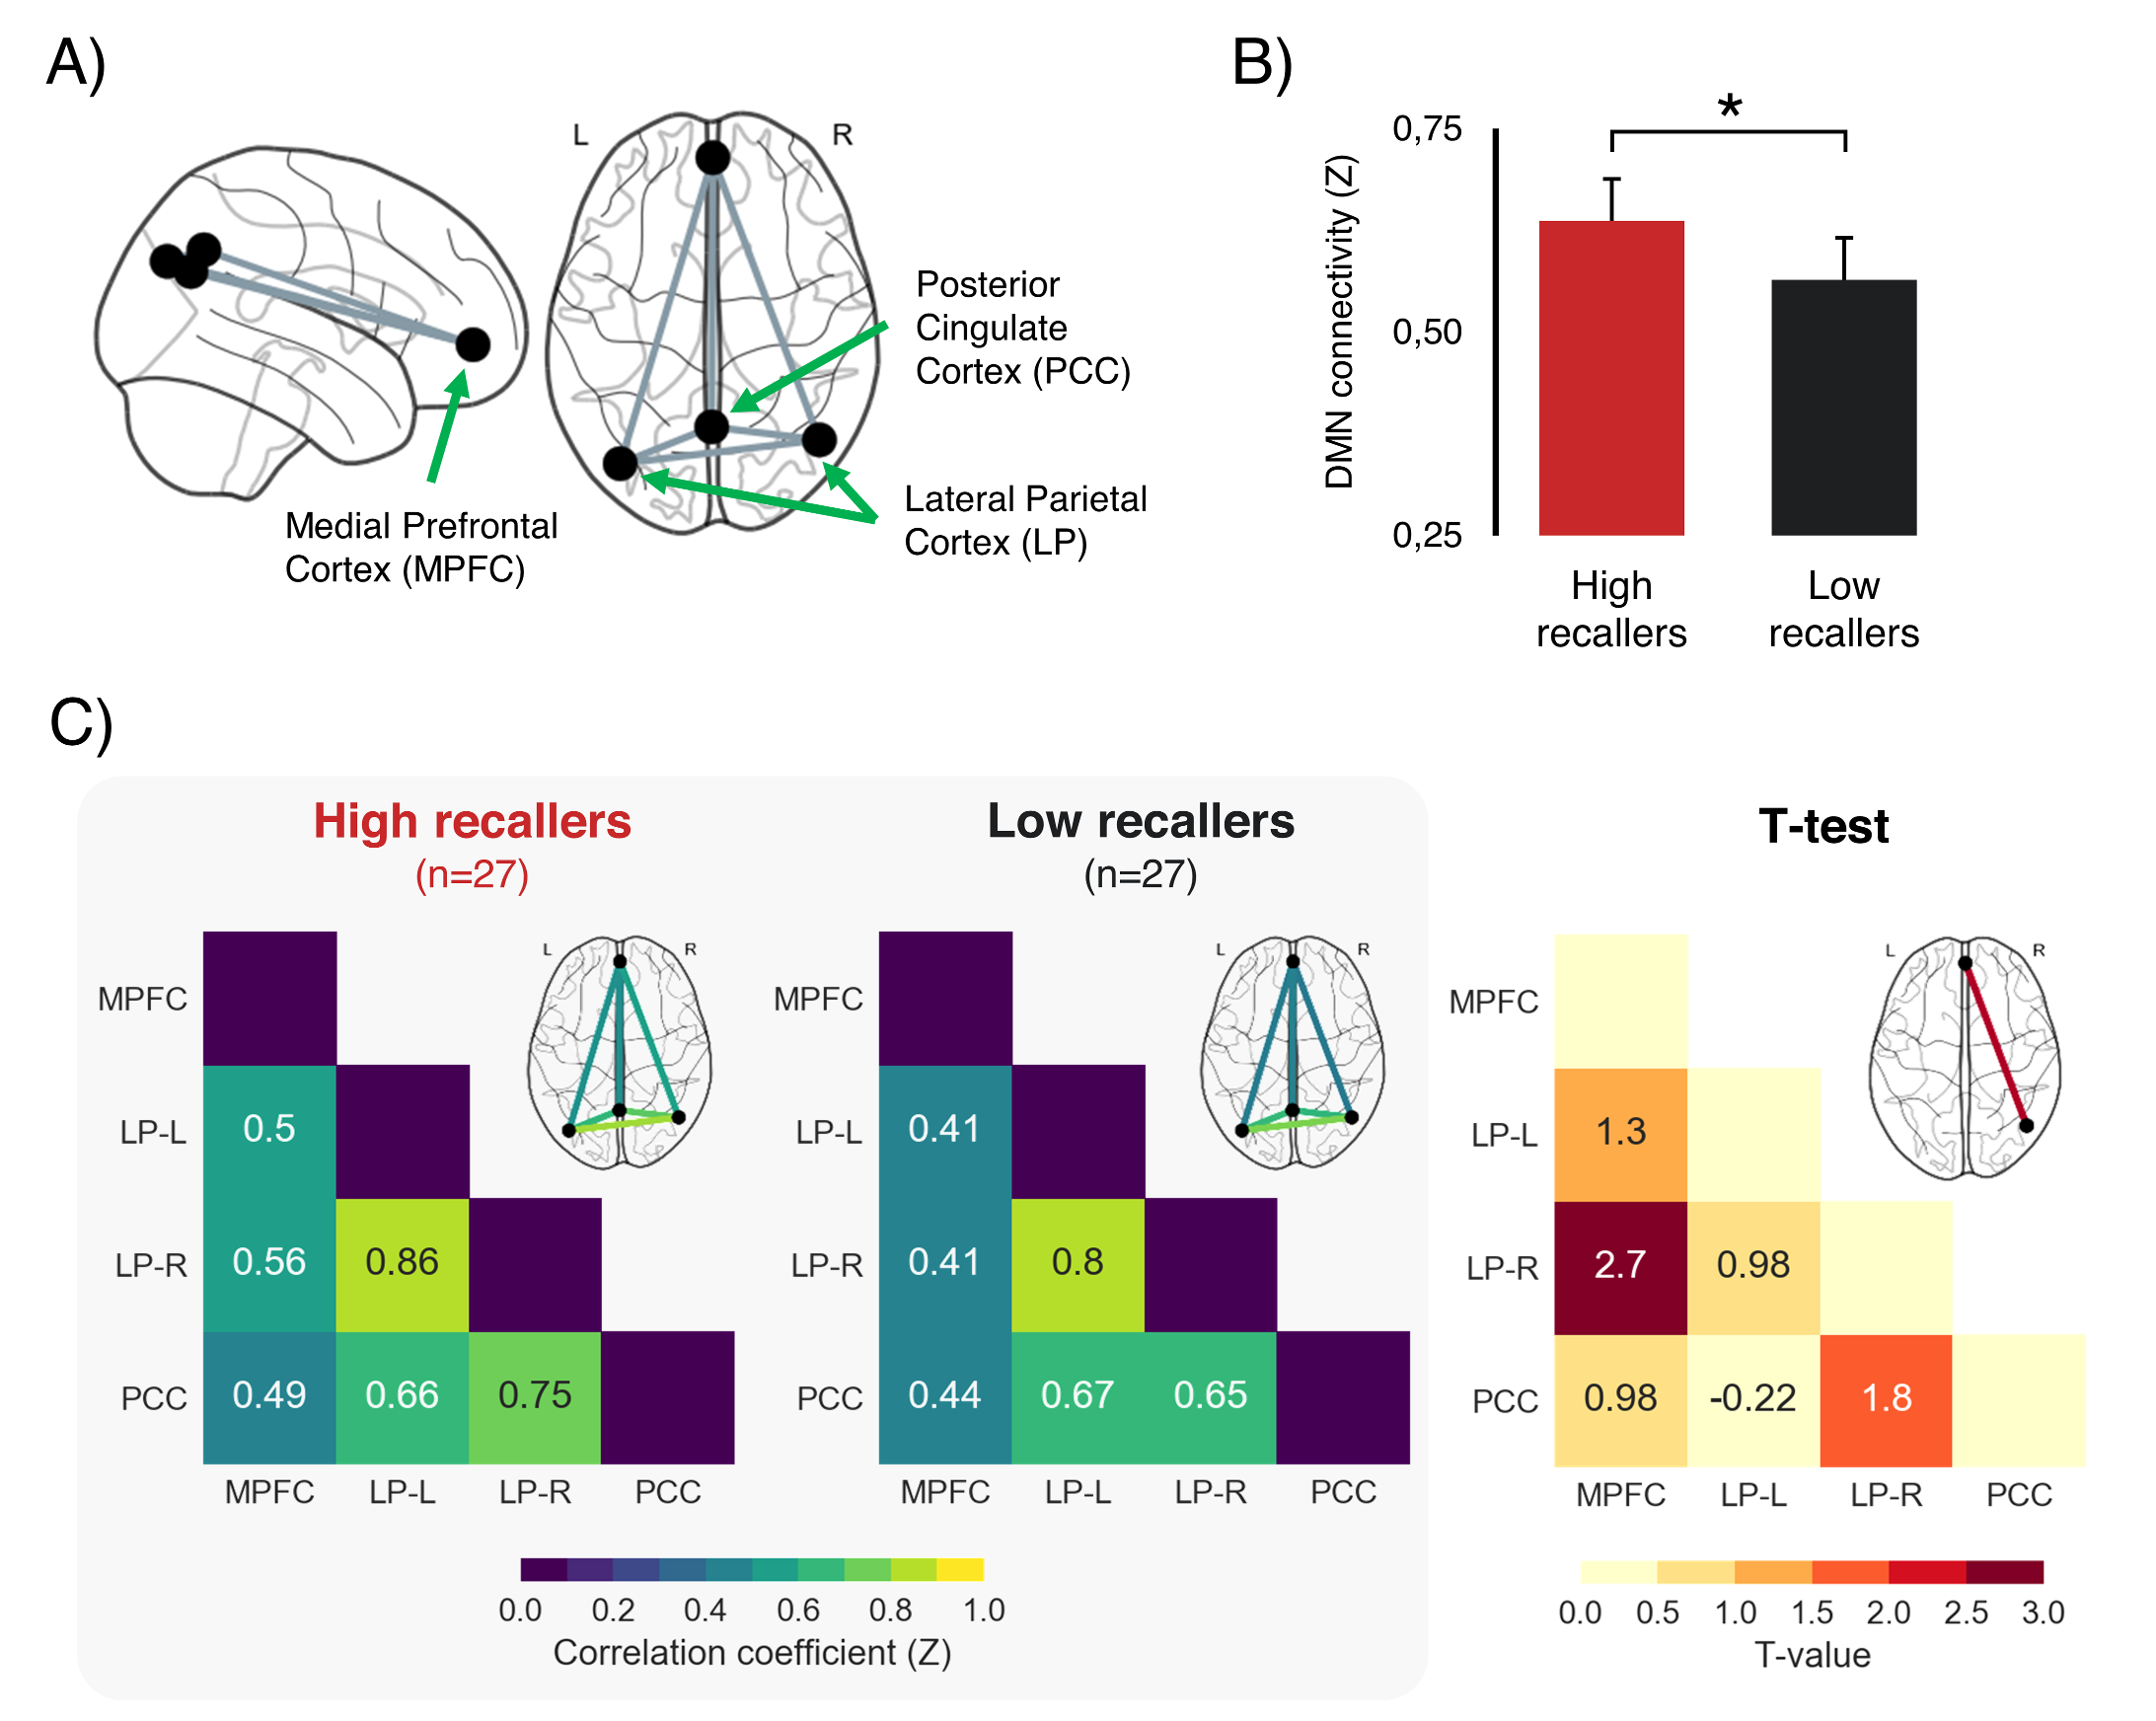
\includegraphics[width=\textwidth]{Fig/Results/Inertia/Creativity/Fig1.png}
	\caption*{\textbf{Fig 1. Increased default mode network connectivity in High dream recallers (HR) compared to Low dream recallers (LR).} (A) Schematic illustration of the four main nodes of the default mode network (DMN) included in further connectivity analysis. (B) Mean pairwise connectivity of the DMN for HR (red) and LR (black), obtained by averaging for each subject all the pairwise correlation values within the default network. The average DMN connectivity was significantly higher in HR than in LR. Error bars represent 95\% confidence intervals. (C) Left grey panel. Functional connectivity matrix representing the mean pairwise correlation coefficient between regions of the DMN in HR and LR. Right. Between-group statistical comparison (two-sided T-test corrected for multiple comparisons using the false discovery rate). The connectivity between the right lateral parietal and medial prefrontal cortex was significantly higher in HR than in LR.}
\end{figure}

\begin{figure}[!htbp]
	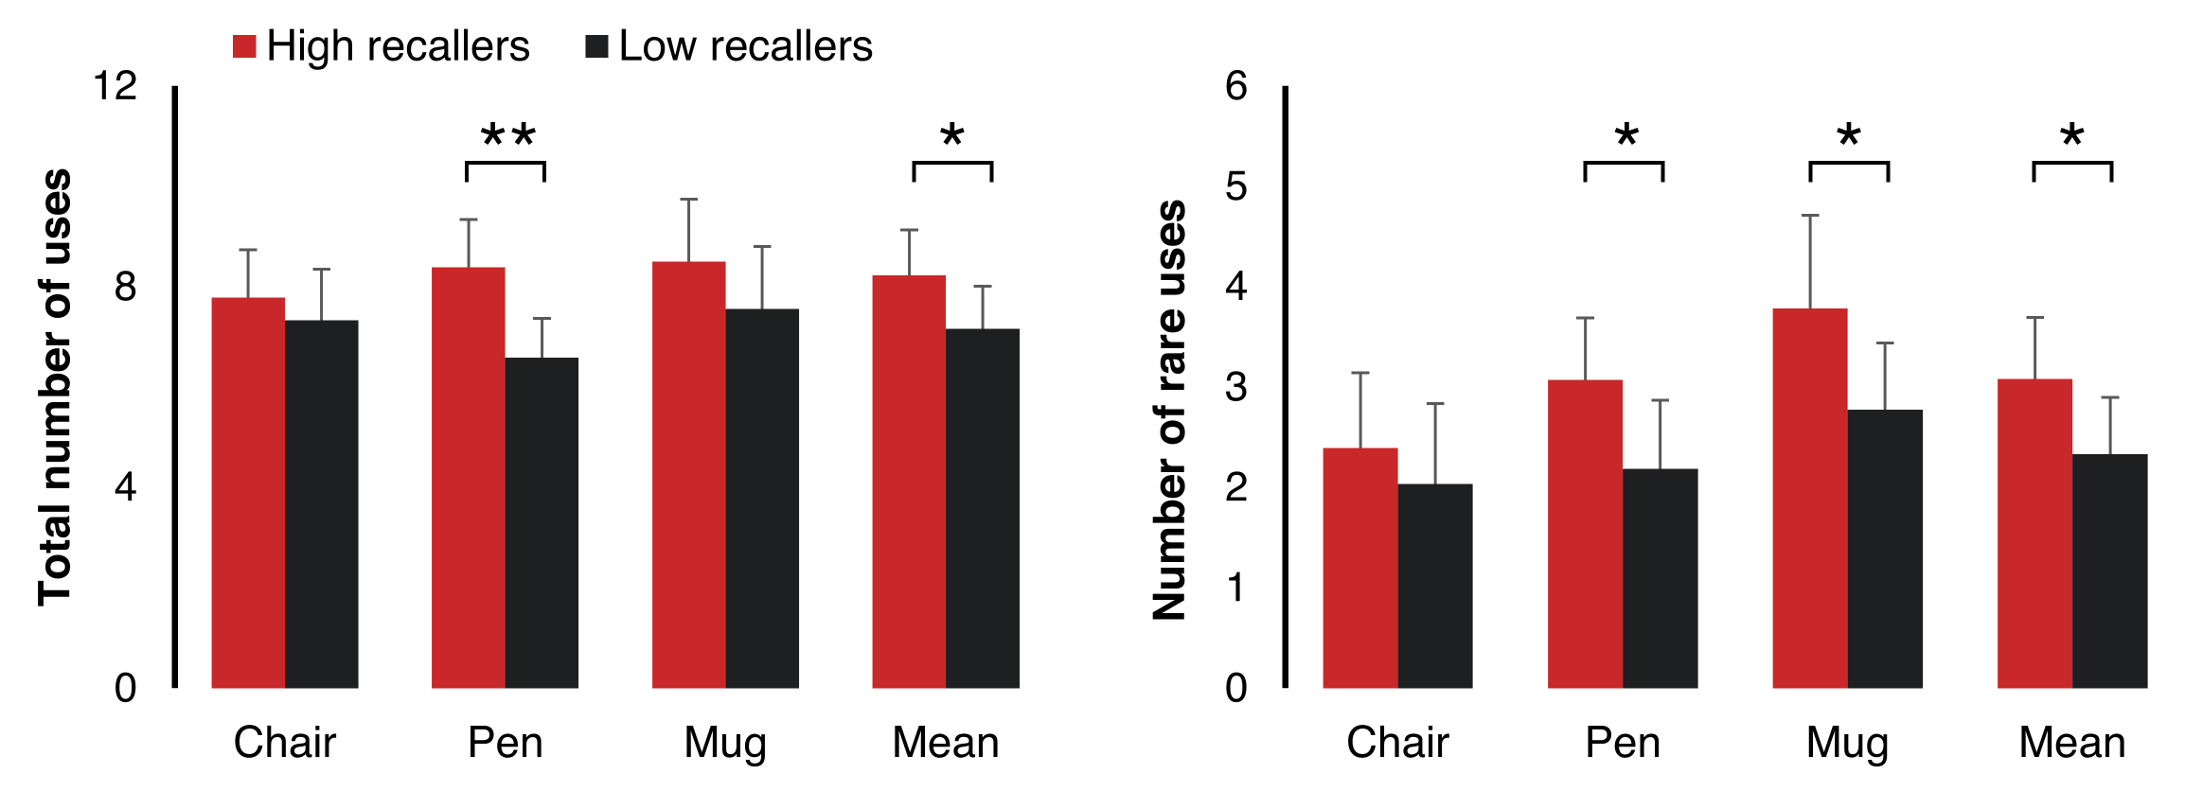
\includegraphics[width=\textwidth]{Fig/Results/Inertia/Creativity/Fig2.png}
	\caption*{\textbf{Fig 2. Higher creativity in High dream recallers (HR) than in Low dream recallers (LR).} \emph{Left}. Group means for the total number of uses found by HR (red) and LR (black) during the Guildford’s alternate uses task. HR reported significantly more uses than LR for the “pen” object and in average (“mean” column). \emph{Right}. Group means for the number of uses reported by 5 or less participants (i.e. top 10\% rarest uses). HR reported significantly more rare uses than LR for the “pen” and “mug” objects, as well as in average (“mean” column). Error bars represent 95\% confidence intervals. *p<.05.}
\end{figure}

% \FloatBarrier

\subsection*{Discussion}
\label{res:dmn-crea:discussion}

This study reports for the first time the brain functional connectivity correlates of DRF in healthy subjects. The results presented above indicate that HR have an increased brain functional connectivity within the DMN, notably between the MPFC and TPJ. In addition HR scored higher than LR on measures of creative-idea generation, without any further between group differences in cognitive or memory abilities.

With regards to functional connectivity, our results are remarkably consistent with a previous PET study from our team that showed, in an unrelated sample of 41 participants, a higher rCBF in HR compared to LR in these two same regions during both sleep and wakefulness \citep{eichenlaub_resting_2014}. Both these studies are in accordance with clinico-anatomical reports showing that lesions in the TPJ and the MPFC lead to a cessation of dream recall \citep{solms_neuropsychology_1997}. Our results provide therefore strong evidence that the ability to recall dreams is linked to rCBF and functional connectivity in these two brain regions.

Furthermore, our findings confirmed previous studies reporting a positive link between creativity and DRF \citep{fitch_variations_1989, schredl_creativity_1995, schredl_factors_2003}. This is of particular interest given that the generation of creative ideas is thought to be also supported by a preferential recruitment of regions of the DMN, and particularly of the MPFC \citep{dietrich_review_2010, ellamil_evaluative_2012, jung_structure_2013, beaty_creativity_2014, mok_interplay_2014, beaty_default_2015}. This large overlap of brain regions involved in dreaming and creativity was noticed by \citet{christoff_mind-wandering_2016} who postulated that creative thought and dreaming are best understood as members \q{of a family of spontaneous-thought processes}. This idea was put slightly differently by \citet{barrett_dreams_2017} who stated that \q{dreaming is essentially our brain thinking in another neurophysiologic state—and therefore it is likely to solve some problems on which our waking minds have become stuck}. Several studies have indeed reported that dream content \emph{per se} often contains solutions of unsolved problems and can be a source of insight \citep{dement_relation_1957, barrett__1993, maquet_psychology:_2004, edwards_dreaming_2013}).

Taking this line of thought further, we argue here that high frequency dream recallers have a specific cognitive and functional profile, involving greater baseline activity in regions of the DMN, which might in turn promote in these individuals creativity and dreaming abilities. Further evidence that HR and LR have a differential neurophysiological profile is provided by recent works from our team showing that HR demonstrated a larger amplitude of brain responses to auditory novel stimuli than LR during both a night of polysomnographically recorded sleep and wakefulness, as well as an increased duration of intra-sleep wakefulness (~15 min more on average) and nocturnal awakenings, whatever of the previous sleep stage, and without any other differences in the micro- or macro-structure of sleep \citep{eichenlaub_brain_2014, vallat_increased_2017}.

Along with the consistent positive association between DRF and creativity, studies have often reported a substantial correlation between DRF and personality traits, such as openness to experience \citep{schredl_dream_2003}, thinner boundaries (i.e. propensity to being more open, trustworthy, vulnerable, and sensitive; \citealp{hartmann_boundaries_1989, schredl_dreaming_1996}), and anxiety \citep{schonbar_manifest_1959, tart_frequency_1962}. None of these variables were statistically different between HR and LR in the present study but it is noteworthy that HR scored higher for all of these variables and some of them were close to significance. Since the above-mentioned correlations have often been reported on larger samples, one can assume that the group differences on these variables would have been significant if our study involved a larger sample of participants. The general idea that differential DRF is linked to traits factors was first introduced by \citet{schonbar_differential_1965} in her so-called \q{life-style} hypothesis. While she did not explained the underlying mechanisms, she postulated that high dream recall is part of a general life style characterized by \q{creativity, rich fantasy, introversion, introspection, field independence and divergent thinking} \citep{schredl_dream_1999}. Our findings argue in favor of this model and provide a brain mechanism for it, i.e. an increased activity in the DMN promoting dreaming and creativity.

Our results suggest that the activity in the DMN should also predict intra-individual variability in DRF across time. This prediction will have to be tested in future studies. DRF enhancing methods (such as keeping a dream diary; \citealp{schredl_questionnaires_2002}) could be indeed used to test whether an increased DRF would result in increased creativity scores and DMN functional connectivity in post compared to pre-training measures within the same individuals (preferentially a group of LR). If true, DRF enhancement methods could become a creativity enhancement method.

% \paragraph{Acknowledgments}
% The authors would like to thank Basak Turker, Morgane Hamon, Franck Lamberton and Danielle Ibarrola for substantial help in data collection and analysis, as well as Jamila Lagha for her help in administrative work.
%
% \paragraph{Author contribution}
% R.V and P.R designed the survey, RV collected, analyzed the data and wrote the first draft. All authors were involved in the writing process.
